\documentclass{chi2009}
\usepackage{times}
\usepackage{url}
\usepackage{graphics}
\usepackage{color}
\usepackage[pdftex]{hyperref}
\usepackage{graphicx}
\usepackage{tabularx}
\usepackage{booktabs}

\newcommand{\docTitle}{Improving Usability of the Linux Kernel Configuration Tools}
\newcommand{\docKeywords}{usability, linux, kernel, configuration}

\hypersetup{%
pdftitle={\docTitle},
pdfauthor={Kacper Bak},
pdfkeywords={\docKeywords},
bookmarksnumbered,
pdfstartview={FitH},
colorlinks,
citecolor=black,
filecolor=black,
linkcolor=black,
urlcolor=black,
breaklinks=true,
}
\newcommand{\comment}[1]{}
\definecolor{Orange}{rgb}{1,0.5,0}
\newcommand{\todo}[1]{\textsf{\textbf{\textcolor{Orange}{[[#1]]}}}}
\newcolumntype{S}{>{\centering\arraybackslash} m{.4\linewidth} }

\pagenumbering{arabic}  % Arabic page numbers for submission.  Remove this line to eliminate page numbers for the camera ready copy

\begin{document}
% to make various LaTeX processors do the right thing with page size
\special{papersize=8.5in,11in}
\setlength{\paperheight}{11in}
\setlength{\paperwidth}{8.5in}
\setlength{\pdfpageheight}{\paperheight}
\setlength{\pdfpagewidth}{\paperwidth}

% use this command to override the default ACM copyright statement 
% (e.g. for preprints). Remove for camera ready copy.
\toappear{Submitted for CS 889 - Open Source Usability.}

\title{\docTitle}
\numberofauthors{2}
\author{
  \alignauthor Kacper Bak\\
    \affaddr{Generative Software Development Lab}\\
    \affaddr{University of Waterloo, Canada}\\
    \email{kbak@gsd.uwaterloo.ca}
  \alignauthor Karim Ali\\
    \affaddr{PLG Group}\\
    \affaddr{University of Waterloo, Canada}\\
    \email{karim@uwaterloo.ca}
}

\maketitle

\begin{abstract}
Tailoring a Linux kernel to one's needs has been one of the most cumbersome tasks a GNU/Linux user can do. There have been many attempts to overcome this problem by introducing smarter configuration tools. Those tools, however, still lack some important features, which discourages users from using them. In this project, we plan to address the problem of usability of the Linux kernel configuration tools. Our aim is to identify the major usability issues with current tools, propose a better user interface and evaluate it on a group of Linux enthusiasts.
\end{abstract}

\keywords{\docKeywords} 

\category{H.5.2}{Information Interfaces and Presentation}{Miscellaneous}%[Optional sub-category]

\section{Introduction}

\section{Problem}\label{sec:problem}

% motivation
Configuration of a big feature model is a laborious process. Users configure kernels to improve stability, apply new bug-fixes, add functionality and drivers. Sometimes it is necessary to upgrade kernel in an embedded system, such as network router or to customize it to specific hardware. Many users configure kernels without even realizing this fact. We distinguish two types of kernel configuration: static and dynamic. The former is the traditional method, where software is customized before compilation. The advantage of this method is smaller program footprint and faster compilation. On the other hand, later reconfiguration requires more effort, because each additional piece of software has to be compiled separately. In many modern distributions users are provided with fully functional kernels, and they do not have to compile themselves. Instead, they dynamically customize the software, by loading relevant modules. The disadvantage of the second method is that preparing such a big kernel takes a lot of time and resources. Furthermore, it is infeasible to apply it to embedded systems. 

% current sw
Regardless of configuration type, there is still need to customize the software. Although this task can be done manually, users prefer to use automated and intuitive tools. Unfortunately, the software currently used for kernel configuration is neither fully automated, nor easy to use. The first claim can be easily verified by creating incorrect configurations that are not reported by the tool. We got to the second conclusion after carrying out an initial study on a group of Linux users.

Linux kernel configurators are targeted to advanced users. Some kernel developers expressed opinion \cite{kernel:aunt:2002} that kernel should be configured only by experienced users. While this statement might be true, there are still lots of Linux novice users who want to learn how to configure kernel or need to compile a particular driver. As of now, there are millions of web pages describing how to configure and compile the Linux kernel. Novice users are often overwhelmed by the number of available options and required knowledge. LKC offers no progressive-disclosure for them.

% initial study
In the first study 6 participants were asked to statically configure the Linux kernel for a popular laptop for typical home or office use. The used the standard \textsf{xconfig} tool that comes with the Linux kernel. A person succeeded if the new kernel was ready to play music and movies, connect to Ethernet, use WiFi, memory cards, USB devices, Bluetooth, CD/DVD. This scenario seemed rather common, because in many Linux distributions users have to fine-tune their configurations to make the whole system work as expected. None of the subjects succeeded with the task without further help. We observed many problems that people had with the tools. We were also interested in how they used \textsf{xconfig}, and how to configure software in general.  \textbf{bleblle}

\begin{description}
  \item[Menu hierarchy]
All participants had problems with selecting drivers for laptop's hardware. First of all, the tool showed the whole hierarchy, and people said they were overwhelmed by thousands of options. Several of them started with collapsing all menus, so that only top-level categories were visible. Furthermore, the tree/sub-tree relationship was confusing. It was unclear whether selection of parent option implies selection of required functionality or additional suboptions should be selected as well. To some, even such a basic thing as checking an option was confusing. Besides familiar empty and filled checkbox, the tool showed a box with dot inside. It meant that the option will be compiled, but as a dynamically loadable module.

  \item[Option names and descriptions]
Cryptic names were another source of problems. The existing infrastructure use names that make sense to programmers and kernel hackers, but are hard to understand for less experienced users. Unfortunately, descriptions were not very helpful, since they often explained implementation details instead of end-user functionality.

  \item[Searching]
Huge hierarchy of options and cryptic names make it very hard to find a particular feature. All participants used search in \textsf{xconfig}. Searching worked very poorly, since feature descriptions were not searched by the tool. People expressed their frustration and often used Google to match modules with hardware, and later select the module in \textsf{xconfig}. Google was also used to find a list of drivers required by the laptop. Arguably, it was easier than running system tools to discover hardware.

  \item[Configuration]
We carefully observed how users used current tools to configure a large piece of software. Most of them were jumping between different categories as they tried to locate modules. One person, who had experience with other tools, started \textsf{menuconfig} program, which performs wizard-like configuration. The problem with this tool was that the user could not jump to other categories, but had to answer many irrelevant questions. When users were unsure about drivers, because 2-3 modules seemed similar, they checked them all. 
\end{description}

% conclusions

The initial study led us to the following conclusions:
\begin{enumerate}
\item Menu hierarchy should be as simple as possible. There are far too many options that could be reduced automatically if the configuration tool targeted specific user group and had good reasoning capabilities.
\item Feature names and descriptions should reflect end-user functionality instead of low-level details.
\item Powerful searching capabilities are crucial as the number of configuration options grows.
\item Automatic hardware detection and kernel autoconfiguration is important, since majority of kernel options is related to hardware drivers.
\end{enumerate}

The aforementioned problems can be fixed by improving application's backend and creating more intuitive user interface. Our project focused on constructing a better user interface that would be intuitive, simple and targeted to specific group of users.

\section{Linux Kernel Configuration Tool}\label{sec:lkc}
% target group

To design such configuration tool, we first set our target group to be less experienced Linux users. In other words, we are building this tool for novice and
intermediate Linux users to allow them to to configure a Linux kernel withouth burdening them with many of the unncessary details involved during such process.
We started the design process of our Linux Kernel Configuration Tool (lkc tool) by designing several mockups that have our vision for the tool. Initially, we
thought that once the tool is started, it should first fetch the current Linux kernel configuration, then detect the currently connected hardware. A dialog box
(splash screen) should be shown to the user at that time to show the progress of these processes. Figure \ref{fig:splash} shows four different mockups for that
dialog box. 

% rationale for the design

\begin{figure*}[!t]
 \centering
\begin{tabular}{SS}
 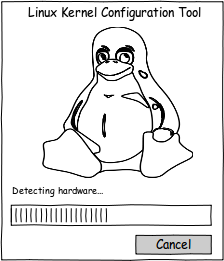
\includegraphics[scale=0.5,keepaspectratio=true]{figs/splash-big.png} & 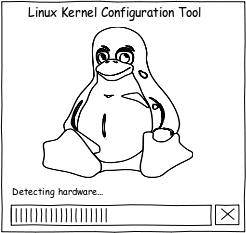
\includegraphics[scale=0.5,keepaspectratio=true]{figs/splash-bigico.png} \\
 (a) & (b) \\
 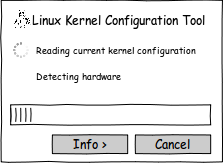
\includegraphics[scale=0.5,keepaspectratio=true]{figs/splash-readingcurrent.png} &
 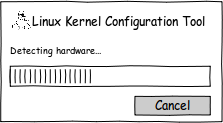
\includegraphics[scale=0.5,keepaspectratio=true]{figs/splash-standard.png} \\
 (c) & (d) \\
\end{tabular}
\caption{Splash screen design mockups}
\label{fig:splash}
\end{figure*}

We decided to do a second user study that included six participants. The aim of this study was to show the participants those designs and get feedback from
them regarding what aspects in those designs were appealing to them, and what were not. That study led us to draw the following conclusions:
\begin{enumerate}
 \item Users always liked to know what is going on. In other words, they did care about getting more information about what the tool is doing while the progress
bars are being filled up.
 \item The fact that users appreciate access to more information does not mean they appreciate that such information should be displayed by default, only when
requested.
 \item It is highly desirable to have the tool report to them any crashes that occur during the hardware detection process.
\end{enumerate}

Consequently, we settled down on the design showin in Figure \ref{fig:splash-final} for our splash screen.

\begin{figure*}[!t]
 \centering
\begin{tabular}{cc}
 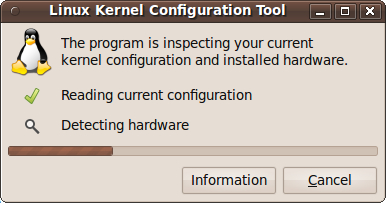
\includegraphics[scale=0.5,keepaspectratio=true]{figs/splash-final1.png} & 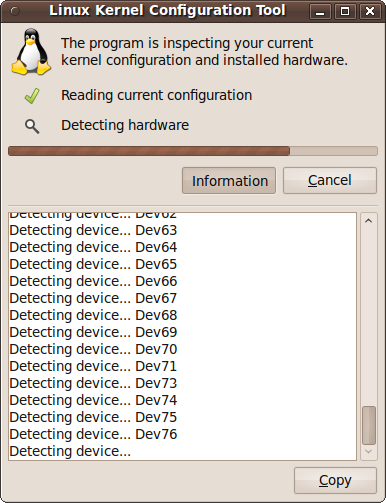
\includegraphics[scale=0.5,keepaspectratio=true]{figs/splash-final2.png} \\
 (a) & (b) \\
\end{tabular}
\caption{Final splash screen design}
\label{fig:splash-final}
\end{figure*}

% xconfig vs lkc

% scalability

% implementation

\section{Evaluation}\label{sec:evaluation}

% participants characterization

\subsection{Threats to Validity}

\paragraph{External Validity}

\paragraph{Internal Validity}

\section{Future Work}\label{sec:futurework}

% \section{Future Work} - we'll place this section in the final report
% \todo{what do you think about creating a graphical tool that goes with you step by step and configures a kernel? basically you answer some questions, press next, and finally click install to install the new kernel. It might be appreciated by beginners. Is it too simplistic? would it be useful? it improves usability, but are there many users who need such a limited tool?}

% backends

\section{Related Work}\label{sec:relatedwork}
% literature review

All the configuration tools are front-ends built on top of a single engine called Linux Kernel Configurator (LKC). LKC analyzes kernel variability and supports users during the configuration stage. LKC uses internally the KConfig language to represent variability and dependencies among features. As several researchers \cite{sincero:lkc:2008,she:kernel:2010} showed, there is a direct correspondence between well-understood feature models and practically crafted variability model used by the Linux kernel. In contrast with formal feature models, LKC is not supported by any formal reasoning engine (e.g. SAT-solver). This is a serious problem, because users can unconsciously create wrong configurations while having no clue why a particular configuration does not work. The Linux kernel community can benefit from adopting well-researched feature models, by making their tools more reliable and eventually usable.

Hardware autodetection and kernel configuration is a recurring problem \cite{debian:config:2010,soft32:config:2007}. Many users complain about the lack of it. The situation is slowly improving as developers added the \textsf{localmodconfig} \footnote{More info at: \url{http://bit.ly/cPgq8R}} target to Linux-2.6.32. The command detects current kernel configuration and applies the same options to the new kernel. It is a step ahead, but the tool is very simplistic and assumes that all the required modules are already loaded. For example, if a computer has built-in Bluetooth, but the module is not loaded, the new kernel will not support the Bluetooth device. Furthermore, the autoconfiguration script offers a very coarse level of options granularity, e.g. if a computer has one sound card, such as Intel HD Audio, the script will select all available sound card drivers and all Intel HD Audio modules. The autoconfiguration tool reads configuration of the running kernel instead of detecting the actual hardware, e.g. for a laptop with the Core Duo 2 processor, it selected 686 processor in the new kernel, because that processor is selected in the running kernel.

Improvements of the configuration tool were already introduced in 2002 when Eric S. Raymond presented the CML2 configuration system \cite{raymond:cml2:2000}. It allowed for effective reasoning on kernel feature model and also provided progressive-disclosure. There was a long debate and flame war about using that system \cite{kerneltrap:linux:2002}. Finally, it was rejected for various reasons, such as Eric S. Raymond's attitude, Python dependency, complexity, radically new design. Many developers preferred to introduce gradual updates instead of applying one big patch.

Debian GNU/Linux device driver check \& report~\cite{muto:check:2010} is an interesting project that helps with matching kernel modules with hardware. It reads output of \textsf{lspci} command, and then outputs driver's name. The project is in fact a big database that stores user's knowledge about the hardware. It could be utilized by the configurator to automatically select relevant modules if devices are hard to discover.

\section{Conclusion}\label{sec:conclusion}

\bibliographystyle{abbrv}
\bibliography{doc}

\end{document}
